%PRESTAR ATENCION: pegado de archivo externo!!!

%ARCHIVO transmitir.tex modificado.

%Dada la motivación, se puede decir a priori que el objetivo del presente trabajo es la implementación de una efectiva comunicación entre una Computadora Personal (PC) y una FPGA. Sin embargo, este objetivo tan amplio se plasmará de forma más concreta y detallada en la Sección \ref{int:obj}.\\

Pero, ¿Cuántos datos son suficientes para el propósito de trasmitir imágenes? ¿Y cuál es el protocolo que mejor se ajusta a la necesidad de disponibilidad? Para responder la primera pregunta, se toma como base de diseño el sensor que utiliza Pérez en su Tesis de Maestría \cite{Perez2018}, una cámara para adquirir imágenes monocromáticas de código MT9M001C12STM, comercializado por Actina Imaging \cite{MicronTechnology2004} que transmite datos a una tasa de \SI{48}{\mega\bit\per\second}.\\

Además, pensando en que la implementación sea compatible con equipos convencionales, es decir, se encuentren fácilmente en el mercado y no posean especificaciones que escapen al uso de oficina. Esto se cumple hoy en día con tres tipos de puertos: Ethernet, dedicado principalmente a conexión de redes mediante cables; Wi-Fi, utilizado para el accesos a la red de forma inalámbrica; y USB, especializado en periféricos.\\

Al hablar de Ethernet o Wi-Fi, se hace referencia a dos formas diferentes de conectarse a una misma cosa: una red de computadoras. En otras palabras, se habla de dos o más nodos, compuestos por PC's o cualquier aparato electrónico con capacidad de realizar cálculo binario, que pueden intercambiar datos a través de una trama bastante compleja de componentes diferentes. Ambos protocolos hacen referencia solo a la conexión física de los dispositivos y el control de acceso de cada uno de ellos a la conexión. Quedando a cargo de otros sistemas, con sus protocolos, que los datos enviados puedan ser correctamente recibidos por el usuario de la PC. La gran diferencia entre ellos radica en el medio físico que utilizan: Wi-Fi emplea ondas electromagnéticas emitidas mediante radiofrecuencia, mientras que en Ethernet, estas ondas son acarreadas por uno o más conductores, como ser cable coaxial, cables de par trenzado o fibra óptica.\\

\begin{figure}
	\centering
	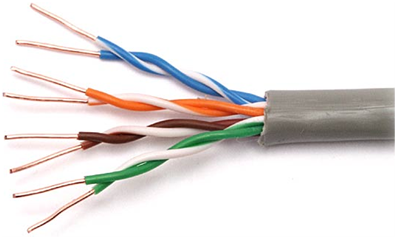
\includegraphics[width=0.4\textwidth]{partrenzado.png}
	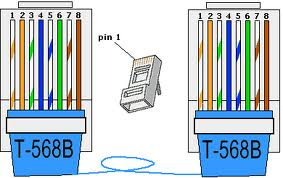
\includegraphics[width=0.4\textwidth]{utp.jpeg}
	\caption{Par Trenzado y un dibujo de su ficha de conexión.}
	\label{fig:utp}
\end{figure}

Ethernet, también conocido como IEEE 802.3, es un protocolo que define cómo se deben conectar nodos a través de conductores para conformar red de área local (LAN o {\it Local Area Network}), es decir, un red pequeña, como ser doméstica, oficina o de una empresa definida, de forma que puedan transmitir información a velocidades a elegir entre \SI{1}{\mega\bit\slash\second} y \SI{400}{\giga\bit\slash\second} \cite{Ethernet2018}. Utiliza una tecnología denominada Acceso Múltiple Sensando la Portadora con Detección de Colisiones (CSMA/CD del inglés {\it Carrier Sense Multiple Access with Collision Detection}), la cual antes de transmitir, corrobora que no exista una señal portadora y, si ésta está presente, espera para retransmitir. Dependiendo de la frecuencia de trabajo y la tasa de transferencia a la que transporta el mensaje, la norma especifica el conector y la distancia máxima a la que debe conectarse una repetidora, es decir, un aparato que reconstruya y emita la señal. Estos conectores pueden ser cable coaxial, fibra optica o cable de par trenzado. Este último es el más usual en las PCs comerciales y se muestra, junto a su ficha característica en la Figura \ref{fig:utp}.\\

La norma IEEE 802.3 también especifica cómo debe ser el formato de la información que se transmite, de forma tal que todas las velocidades, conectores y conductores sean compatibles entre si. La información se intercambia contenida en paquetes cuya estructura permite la comunicación entre muchos nodos de la red. La trama está compuesta por \SI{7}{\byte} de preámbulo que sirve para sincronizar los extremos de la conexión, un byte de inicio, 12 de direcciones, que corresponden 6 al nodo emisor y 6 al destinatario respectivamente, dos que indican la longitud del mensaje, entre 46 y \SI{1500}{\byte} de datos y, finalmente, 4 de verificación. Otra definición importante de la norma, son las características eléctricas de las señales, pero no se detallan en este trabajo porque varían en función de la velocidad del puerto.\\

Por su parte Wi-Fi, perteneciente a la asociación de compañías denominada Wi-Fi Aliance, se rige por la norma que estableció esta última. Existe una norma equivalente, encuadrada en la especificación IEEE 802.11, referida a las redes de area local inalámbrica, o WLAN (siglas del ingles {\it Wireless Local Area Network}). Wi-Fi se enfoca en las que se refieren a las comunicaciones de radiofrecuencia con portadora de \SI{2,4}{\giga\hertz}, que se incorporan en las revisiones b, g y n de la norma IEEE. IEEE 802.11 está pensado especialmente para dispositivos portátiles y móviles, que según la norma, los primeros aparatos, si bien pueden moverse con facilidad, operan estáticos, y los segundos trabajan en movimiento \cite{wifi2016}. La principal característica que posee es la falta de conductores para la elaboración de la red, más que las conexiones entre los transceptores (emisores y receptores de radiofrecuencias) y los nodos. En cuanto a la trama que utiliza para enviar y recibir datos es muy similar a la de un puerto Ethernet.\\

Existen múltiples ventajas de utilizar radiofrecuencias para conectarse a la red, tales como la libertad de mover el punto de trabajo y la economía a la hora de armar redes con muchos nodos. Sin embargo, posee algunas desventajas notorias, propias del medio de propagación, que lo hacen no tan óptimo para los fines del presente trabajo. Las redes inalámbricas tiene la característica de que no es del todo confiable: posee múltiples fuentes de interferencia, ya que varias tecnologías que utilizan la misma frecuencia (Bluetooth, Zig-Bee, WUSB, microondas). Esto hace que la señal por momentos presente cierta interferencia. A su vez, suele presentar variaciones temporales y asimetrías en las propiedades de propagación, lo que puede provocar interrupciones en la comunicación.\\

Ambos protocolos proporcionan una solución de conexión de redes de nivel físico y ejecutan tareas de control de acceso al medio (MAC) a fin de evitar colisión en los datos, es decir, que dos dispositivos transmitan en forma simultánea e interfieran la comunicación.
Sin embargo, para establecer una red, faltan componentes físicos y lógicos tales como un sistema de control enlace lógico (Logic Link Control), un sistema de direccionamiento, como el Protocolo de Internet (IP), una capa de transporte de datos, (como el protocolo TCP) y las capas de software que permiten acceder a los protocolo anteriormente mencionados.\\

A pesar de lo anterior, es posible establecer comunicaciones punto a punto con ambos protocolos, simplificando mucho el sistema de transmisión de datos. Sin embargo esta solución presenta un inconveniente no menor: se le quita a la PC un acceso a la red, que en la mayoría de los casos es el único. Esto no es deseable ya que la conectividad es un requisito fundamental en cualquier hogar u organización, ya sea empresarial, gubernamental, científica o de cualquier tipo.\\

Por su parte el protocolo USB (acrónimo de {\it Universal Serial Bus}), es una norma desarrollada por seis de las empresas más grandes de la industria informática, pensada y desarrollada para la conexión de teléfonos y periféricos a PCs \cite{USBspec}. En la versión original, USB poseía conectores cableados de 4 conductores, y presenta una topología de bus, es decir todos los dispositivos conectados a una misma conexión física, que es manejada por una PC y en la cual solo transmite y recibe un dispositivo a la vez. Este tipo de conexión tuvo tal penetración en el mercado que se trasnformó en una norma de facto y actualmente es incorporada casi por defecto y necesaria a la hora de comprar e instalar periféricos.\\
%Si bien se puede implementar la comunicación vía Ethernet, cumpliendo con las especificaciones propuestas, es muy probable que el único puerto que posea la PC se encuentre conectado a la red y se necesitará una infraestructura mayor para lograr una efectiva comunicación. Por tanto, USB se observa como una solución óptima.\\

USB presenta diferentes versiones de su norma, cada cual con una o más tasas de transmisión y señalización. La versión 1 posee dos revisiones, 1.0 fue lanzada al mercado en el año 1996 y 1.1 que se presentó en Agosto de 1998. La primera alcanza una tasa máxima de \SI{1.5}{\mega\bit\per\second} y la segunda hasta \SI{12}{\mega\bit\per\second}. USB 2.0 fue presentado en Septiembre del 2000 y es capaz de transmitir a \SI{480}{\mega\bit\per\second}. La tercera versión, USB 3.0, fue lanzada al mercado en 2011 y transmite \SI{5}{\giga\bit\per\second}. Esta última versión fue revisada en julio de 2013 y en septiembre de 2017, ofreciendo la primera de ella \SI{10}{\giga\bit\per\second} y \SI{20}{\giga\bit\per\second} la segunda. Resulta suficiente para el propósito del siguiente trabajo, la implementación de una comunicación USB 2.0, con tasa de transferencia de \SI{480}{\mega\bit\per\second}.\\

\begin{figure}[t]
	\centering
	\begin{tikzpicture}[scale=\textwidth/\paperwidth,>=latex]
	\begin{scope}
	\begin{scope}[transform shape,node distance=2]
	\node[bloque]	(cy)					{Interfaz};
	\node[bloque]	(fpga)	[right=of cy]	{FPGA};
	\node[bloque]	(pc) 	[left=of cy]	{PC};
	\draw[->,thick]	(pc.15)	-- node (usbd+) [above]	{D+} (pc.15 -| cy.west);
	\draw[->,thick]	(cy.195)-- node (usbd-) [below]	{D-} (cy.195 -| pc.east);
	\draw[<->,thick](cy.15) -- node (data) [above] {Datos} (cy.15 -| fpga.west);
	\draw[->,thick]	(fpga.195)	-- node (ctrl) [below]	{Control} (fpga.195 -| cy.east);
	\node[node distance=.4]	(usb text) [above=of usbd+]	{USB};
	\end{scope}
	\begin{scope}
	\node[rectangle,rounded corners,draw=black,dashed,fit=(usb text)(usbd+)(usbd-)(cy.south west)(pc.east)](usb){};
	\end{scope}
	\end{scope}
	\end{tikzpicture}
	\caption{Esquema propuesto para implementar la comunicación}
	\label{fig:esq}
\end{figure}

El alumno sabe que es posible implementar una comunicación USB completa a través de una FPGA. Sin embargo, esto sería muy costoso en términos de tiempos de desarrollo y de recursos de FPGA disponibles para la implementación de otros sistemas, los cuales son el objetivo de la comunicación.\\

Se plantea, entonces, un esquema como el que se observa en la Figura \ref{fig:esq} en la cual se utiliza una interfaz externa al FPGA. La comunicación USB propiamente dicha será efectuada entre la interfaz y la PC, mientras que se plantea una comunicación diferente entre la interfaz y el FPGA. Este último, por su parte, tendrá la tarea de realizar el control de esta comunicación.\\

%Atención con estos parrafos!!!!

%
% una tasa de bit que permita transmitir imagenes y que los puertos sean fácilmente accesibles en PCs comerciales, resaltan tres protocolos que permitirían lograr este cometido: Ethernet, USB y Wi-Fi. Estos protocolos, son los que actualmente se encuentran presente en cualquier aparato nuevo. Estas normas, entre otras, han dejado de lado a estandares que antes eran muy comunes y que algunos periféricos aún cuentan, como ser RS-232 o PS/2, entre otras.\\ 
%
%En una primera aproximación, la que mayor tasa de datos puede proveer, sin dudas es el estandar Ethernet. Estas comunicaciones pueden alcanzar hasta \SI{400}{\giga bp\second}. Sin embargo, la norma Ethernet está principalmente pensada para redes de computadoras, por lo general se dipone de un solo puerto, el cual puede estar conectado a una red de internet y un periférico que tenga este puerto como conexión requerirá de alguna infrastructura adicional con cables más o menos extensos para lograr la comunicación.\\
%
%En el caso de tratar de utilizar una comunicación via Wi-Fi, es posible que se necesite algún enrutador adicional a la hora de conectarse. A su vez, la tecnología inalámbrica con mayor ancho de banda está disponible hace unos pocos años y no todos los equipos cuentan con esta posibilidad, ofreciendo en esos casos una tasa máxima de \SI{54}{\mega bp \second}. La tasa de transmisión real máxima, descontando todos los encabezados y las colas que posee la norma, es de \SI{19}{\mega bp\second}.

%ARCHIVO
